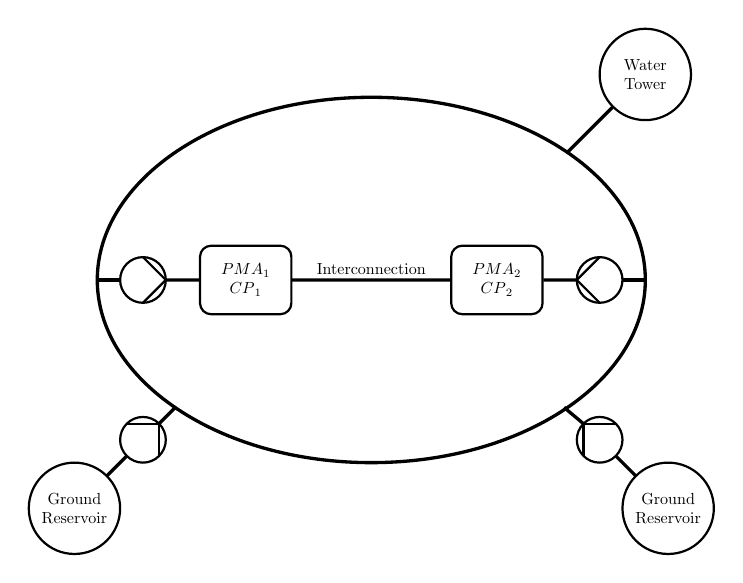
\begin{tikzpicture}[scale=0.58,transform shape]
\tikzstyle{box} = [draw,thick,rounded corners, minimum height=15mm, minimum width=20mm, align=center, text centered]
%Main Ring
\draw[very thick] (7,5.5) ellipse (6 and 4);
%Pump
\draw[thick,transform shape] (2,5.5) circle (0.5);
\draw[thick,transform shape] (2.5,5.5) -- (2,6);
\draw[thick,transform shape] (2.5,5.5) -- (2,5);
%Pump
\begin{scope} [rotate around={180:(12,5.5)}]
\draw[thick,transform shape] (12,5.5) circle (0.5);
\draw[thick,transform shape] (12.5,5.5) -- (12,6);
\draw[thick,transform shape] (12.5,5.5) -- (12,5);
\end{scope}
%Pump
\begin{scope} [rotate around={135:(12,2)}]
\draw[thick,transform shape] (12,2) circle (0.5);
\draw[thick,transform shape] (12.5,2) -- (12,2.5);
\draw[thick,transform shape] (12.5,2) -- (12,1.5);
\end{scope}
%Pump
\begin{scope} [rotate around={45:(2,2)}]
\draw[thick,transform shape] (2,2) circle (0.5);
\draw[thick,transform shape] (2.5,2) -- (2,2.5);
\draw[thick,transform shape] (2.5,2) -- (2,1.5);
\end{scope}
%Reservoirs
\node[thick,draw,circle,minimum width=20mm,align=center] (R1) at (0.5,0.5) {Ground \\ Reservoir};
\node[thick,draw,circle,minimum width=20mm,align=center] (ER1) at (13,10) {Water \\ Tower};
\node[thick,draw,circle,minimum width=20mm,align=center] (R2) at (13.5,0.5) {Ground \\ Reservoir};
%PMA and interconnection
\node[box] (PMA1) at (4.25,5.5) {$\text{PMA}_1$ \\ $\text{CP}_1$};
\node[box] (PMA2) at (9.75,5.5) {$\text{PMA}_2$ \\ $\text{CP}_2$};
\draw[very thick](PMA1) -- (PMA2);
\node[align=center] (PMAc) at (7,5.75) {Interconnection};
%Connections
\draw[very thick](1.2,1.2) -- (1.65,1.65);
\draw[very thick](2.34,2.34) -- (2.71,2.71);
\draw[very thick](12.8,1.2) -- (12.36,1.64);
\draw[very thick](11.66,2.34) -- (11.22,2.71);
\draw[very thick](13,5.5) -- (12.5,5.5);
\draw[very thick](11.5,5.5) -- (PMA2);
\draw[very thick](1,5.5) -- (1.5,5.5);
\draw[very thick](2.5,5.5) -- (PMA1);
\draw[very thick](12.28,9.28) -- (11.29,8.29);
\end{tikzpicture}